\documentclass[12pt, letterpaper]{article}
\usepackage{amsmath}
\usepackage{pgfplots}
\pgfplotsset{compat=1.17} % or any latest version you have
\usepackage{graphicx} % Required for inserting images\documentclass{article}

\title{15 Maximum and Minimum Values (Extrema)}
\author{Damiam Alfaro}
\date{December 2023}

\begin{document}

\maketitle

\section{Maximum and Minimum Values Part A}
\textbf{Motivation}: Optimization problems appear in many applicatons; their solution usually hinges upon finding extreme values of functions.\\
\newline
\textbf{Goal}: Understand how extreme values of functions on closed intervals occur either at the endpoints or at critical numbers.\\
\newline

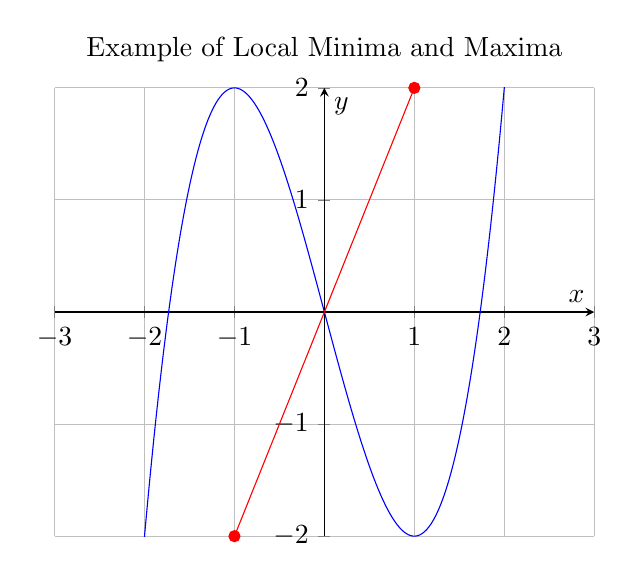
\begin{tikzpicture}
\begin{axis}[
    title={Example of Local Minima and Maxima},
    xlabel={$x$},
    ylabel={$y$},
    xmin=-3, xmax=3,
    ymin=-2, ymax=2,
    grid=both,
    axis lines=middle
]

% Add your function here
\addplot[domain=-2.5:2.5, samples=100, smooth, blue] {x^3 - 3*x};

% Add points for local minima and maxima
\addplot[mark=*, red, mark options={scale=1}] coordinates {(-1,-2) (1,2)};

\end{axis}
\end{tikzpicture}\\
\newline
Basically, the local minimum is at \([-1,-2]\) and the local maximum is at \([1,2]\).\\
\newline
A function can have infinite local minimum and maximum, however, when the function is put within the boundaries of an interval, i.e. \([a,b]\), then it might only contain a few local maximum and minimum.\\
\newline
One can attempt the \underline{Fermat's Theorem}: If \(f\) has a local maximum or minimum at \(x=c\) then \(\frac{d}{dx} f(c)\) either doesn't exist or \(\frac{d}{dx} f(c) = 0\). For example:\\
\newline
\(f(x)=2x^3+3x^2-12x+2\) Defined for x in \([-3,2]\)\\
\newline
The only numbers \(c\) that will give you \(f'(c) = 0\) correspond to the local maximum and local minimum. Those are Maximum: \(c = -2\) and Minimum: \(c=1\).
\[f'(x) = 6x^2+6x-12\]
\[f'(x) = 6(-2)^2+6(-2)-12 = 0\]
\[f'(x) = 6(1)^2+6(1)-12 = 0\]
For a \(f\) function defined in \([a,b]\); c in \((a,b)\) is a \underline{critical number} of \(f\) if \(f'(c)=0\) or \(f'(c)\) does not exist. This means that a function can only have a local extreme value at a critical number.\\
\newline
If they give you a function \(f\) that is defined in \(-\infty, \infty\), i.e. all real numbers, all scenarious, you will need to find where \(c = 0\) or undefined by solving for \(x\) for the given function, this is useful to calculate critical points in operation research:
\[f(x) = (x-4)^{\frac{2}{3}}; (-\infty,\infty)\]
Solve for \(x\) using the chain rule in this case:
\[f'(x) = \frac{2}{(3)(\sqrt[3]{x-4})}\]
As you can see, the function will be \textit{undefined} if we input \(f'(4)\). Therefore we only have one critical number here: \(c = 4\). However, there will be times where a \(f'(c) = 0\) doesn't mean a critical point, but an inflection point:
\[f(x) = x^3\]
\[f'(x) = 3x^2\]
\[f'(0) = 0\]
Happy right? Wrong. Look at its graph.
\begin{center}
\begin{tikzpicture}
\begin{axis}[
    axis lines = middle,
    xlabel = \(x\),
    ylabel = {\(x^3\)},
    xmin=-2, xmax=2,
    ymin=-8, ymax=8,
]
% Plotting the function x^3
\addplot [
    domain=-2:2, 
    samples=100, 
    color=red,
] {x^3};
\end{axis}
\end{tikzpicture}
\end{center}
It just stops momentarily but then keeps increasing exponentially, be careful.\\
\newline
A function can have both; a quotient with \(f'(c) = 0\) at either the numerator or denominator and viceversa, and the same for \(f'(c) =\) undefined.\\
\newline
\[f(x) = 6x^{\frac{2}{3}}+x^{\frac{5}{x}}\]
\[f'(x) = \frac{4+\frac{5}{3}x}{x^{\frac{1}{3}}}\]
On the top, the critical number is \(x=-\frac{12}{5}\) if you solve for \(0\), giving \(f'(c) = 0\). And on the bottom the critical number is \(x=0\), giving \(f'(c)=\) undefined.

\section{Global Maximum and Minimum Values}
\textbf{Motivation}: Optimization problems appear in many applications; their solution usually hinges upon finding extreme values of functions.\\
\newline
\textbf{Goal}: Understand how extreme values of functions on closed intervals occur either at the endpoints or at critical numbers.\\
\newline
\underline{Corollary of Fermat's Theorem}: A critical point that happens to be the boundary of an interval is not to be counted as a critical point.\\
\newline
In order to find the absolute maximum and minimum one has to compare all given numbers and see which of them "scores" higher. 
\[f(x) = 2x^3+21x^2-48x+1; [-8,2]\]
Find the zeros or undefined, aka critical numbers:
\[f'(x)=6x^2+42x-48\]
\[6x^2+42x-48=0\]
\[6(x^2+7x-8)=0\]
\[6(x+8)(x-1)=0\]
As we can see, two critical points are \(x=-8\) and \(x=1\), however, since \(-8\) happens to be a boundary in the interval, we ignore it as critical point. Now we compare the numbers and see which one scores higher, input all the numbers to the initial \(f(x)\):
\begin{center}
\begin{tabular}{c|c}
    \hline
    CV: x = 1 & f(1) = -24\\
    \hline
    a: x = -8 & f(-8) = 705\\
    \hline
    b: x = 2 & f(2) = 5\\
    \hline
\end{tabular}
\end{center}
Now, the bigger score is \(705\), which is the absolute maximum. The smallest score is \(-24\), that is the absolute minimum.\\
\newline
If you get a negative value or positive value that is \underline{out site the given interval}, \underline{ignore it}.\\
\newline
\textbf{Theorem: First Derivative Test}: Let \(c\) be a critical number of the function \(f\): if \(f'(x) > 0 \) to the left of \(c\) and \(f'(x)<0\) to the right of \(c\), then \(f\) has a relative maximum at \(c\).\\
\newline
If \(f'(x) < 0 \) to the left of \(c\) and \(f'(x)>0\) to the right of \(c\), then \(f\) has a relative minimum at \(c\).\\
\newline
If \(f'(x)\) has the same sign on both sides of \(c\), then \(f\) has neither of those at \(c\). For example:
\[f(x)=2x^3-24x+5; (-\infty, \infty)\]
\[f'(x)=6x^2-24\]
For \(f'(x) = 0\), we get that the critical points are \(\pm 2\):
\begin{center}
\begin{tabular}{c|c|c|c}
    \hline
    x & 1 & 2 & 3\\
    \hline
    f'(x) & -18 & 0 & 30\\
    \hline
\end{tabular}
\end{center}
Here we can see that to the left of \(c\) \(f'(x) < 0\) and to the right of \(c\) \(f'(x) > 0\), which is the local minimum.
\begin{center}
\begin{tabular}{c|c|c|c}
    \hline
    x & -3 & -2 & -1\\
    \hline
    f'(x) & 30 & 0 & -18\\
    \hline
\end{tabular}
\end{center}
Here we can see that to the left of \(c\) \(f'(x) > 0\), which is the local minimum, and to the right of \(c\) \(f'(x) < 0\), which is the local maximum.  Why local? Because the interval is all real numbers, therefore we don't know how many there are.\\
\newline
\textbf{Theorem}: If \(f\) is a continous function on \((a,b), [a,b), or (a,b]\) and \(f\) has solely one critical number \(c\) in the interval, and if \(f\) has a local minium at \(c\), then \(f\) has its absolute minimum at that value \(c\), \(f(c)\). The same goes for if \(f\) has a local maximum there with solely one critical number, then it means \(f(c)\) is the local maximum.\\
\newline
Find the \underline{local} and \underline{absolute extreme values} for the following example on interval \((0,\infty)\):
\[f(x)=5x\ln{x}-9x\]
First you find the derivative to find critical values using the product rule in this case, however, the critical value cannot be \(0\) since \(0\) isn't included in the interval:
\[f'(x)=(5\ln{x}+\frac{5x}{x})-9\]
\[f'(x)=5\ln{x}+5-9\]
\[f'(x)=5\ln{x}-4\]
Now you solve for x
\[0=5\ln{x}-4\]
\[4=5\ln{x}\]
\[\frac{4}{5}=\ln{x}\]
\[e^{\frac{4}{5}}=x\]
We apply the first derivative test to check if the new found critical number \(e^{\frac{4}{5}}\) is a local maximum or minimum, recall that the interval is \((0, \infty)\):\\
\begin{center}
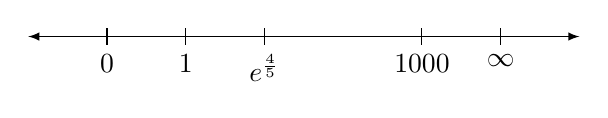
\begin{tikzpicture}
    % Draw the number line
    \draw[latex-latex] (-1,0) -- (6,0); 
    % Mark the points
    \draw[shift={(0,0)},color=black] (0pt,3pt) -- (0pt,-3pt) node[below] {$0$};
    \draw[shift={(1,0)},color=black] (0pt,3pt) -- (0pt,-3pt) node[below] {$1$};
    \draw[shift={(2,0)},color=black] (0pt,3pt) -- (0pt,-3pt) node[below] {$e^{\frac{4}{5}}$};
    \draw[shift={(4,0)},color=black] (0pt,3pt) -- (0pt,-3pt) node[below] {$1000$};
    \draw[shift={(5,0)},color=black] (0pt,3pt) -- (0pt,-3pt) node[below] {$\infty$};
\end{tikzpicture}
\end{center}
As you can see, the two extremes are \(0, \infty\), in the middle we have our \(c\). If we input \(1\) to the derivative function \(f'(x)=5\ln{x}-4\), as is permissible since is within the interval, and is to the left of \(c\), we get a negative number:
\[f'(1)=5\ln{1}-4 = -4\]
If we plug in any number to the right of \(c\)-any number because we have \(\infty\) as our boundary, therefore \(1000\), we get a positive number. Therefore \(f'(x) < 0 \) to the left of \(c\) and \(f'(x)>0\) to the right of \(c\) applies, meaning local minimum.\\
\newline
Now using our previous Theorem, we know that this is the solely critical number, therefore this local minimum is also a global minimum.\\
\newline
To find \underline{Absolute extreme values}, we plug our \(c\) to the initial function:
\[f(e^{\frac{4}{5}})=5(e^{\frac{4}{5}})\ln{(e^{\frac{4}{5}})}-9(e^{\frac{4}{5}})\]
\[f(e^{\frac{4}{5}})= -5e^{\frac{4}{5}}\]



Stupidity is better to keep a secret than displayed.
-Heraclitus, Fragments



\end{document}






\end{document}
